\documentclass{article}

\usepackage{tikz}
\usetikzlibrary{positioning,matrix,calc,backgrounds}

\tikzset{block/.style={draw,circle}}

\begin{document}

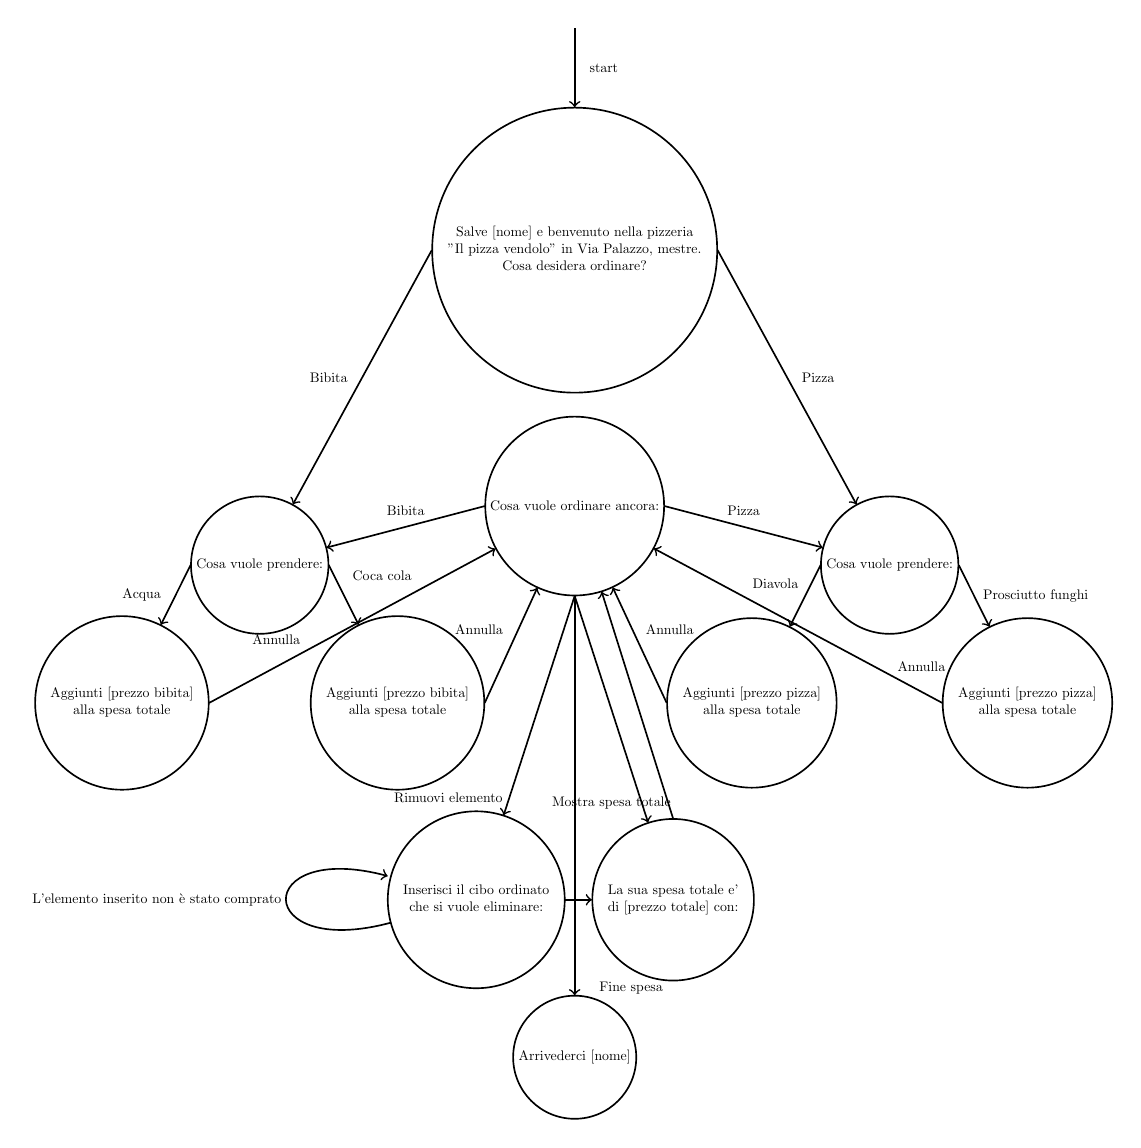
\begin{tikzpicture}[-stealth, on grid, node distance=1cm, scale=0.5, semithick, transform shape]

% Blocchi
\node [block] (start) {
    \begin{tabular}{cc}
        Salve [nome] e benvenuto nella pizzeria \\
        "Il pizza vendolo" in Via Palazzo, mestre. \\
        Cosa desidera ordinare?
    \end{tabular}
};
\node [block, below left=8cm and 8cm of start] (Bibita) {
    Cosa vuole prendere:
};
\node [block, below right=8cm and 8cm of start] (Pizza) {
    Cosa vuole prendere:
};
\node [block, below=6.5cm of start] (Annulla) {
    Cosa vuole ordinare ancora:
};
\node [block, below left=3.5cm and 3.5cm of Bibita] (Acqua) {
    \begin{tabular}{cc}
        Aggiunti [prezzo bibita]\\
        alla spesa totale
    \end{tabular}
};
\node [block, below right=3.5cm and 3.5cm of Bibita] (CocaCola) {
    \begin{tabular}{cc}
        Aggiunti [prezzo bibita]\\
        alla spesa totale
    \end{tabular}
};
\node [block, below left=3.5cm and 3.5cm of Pizza] (Diavola) {
    \begin{tabular}{cc}
        Aggiunti [prezzo pizza]\\
        alla spesa totale
    \end{tabular}
};
\node [block, below right=3.5cm and 3.5cm of Pizza] (ProsciuttoFunghi) {
    \begin{tabular}{cc}
        Aggiunti [prezzo pizza]\\
        alla spesa totale
    \end{tabular}
};
\node [block, below left=10cm and 2.5cm of Annulla] (RimuoviElemento) {
    \begin{tabular}{cc}
        Inserisci il cibo ordinato\\
        che si vuole eliminare:
    \end{tabular}
};
\node [block, below right=10cm and 2.5cm of Annulla] (MostraSpesaTotale) {
    \begin{tabular}{cc}
        La sua spesa totale e' \\
        di [prezzo totale] con:
    \end{tabular}
};
\node [block, below=14cm of Annulla] (FineSpesa) {Arrivederci [nome]};

%Collegamenti
\path[->] ($(start.north)-(0,-2)$) edge node[right=0.25cm] {start} (start.north);
\path[->] (start.west) edge node[left=0.25cm] {Bibita} (Bibita);
\path[->] (start.east) edge node[right=0.25cm] {Pizza} (Pizza);
\path[->] (Bibita.west) edge node[left=0.25cm] {Acqua} (Acqua);
\path[->] (Bibita.east) edge node[above right=0.25cm and 0.10cm] {Coca cola} (CocaCola);
\path[->] (Pizza.west) edge node[above left=0.05cm and 0.05cm] {Diavola} (Diavola);
\path[->] (Pizza.east) edge node[right=0.10cm] {Prosciutto funghi} (ProsciuttoFunghi);
\path[->] (Acqua.east) edge node[below left=0.10cm and 1.2cm] {Annulla} (Annulla);
\path[->] (CocaCola.east) edge node[above left=0.15cm and 0.08cm] {Annulla} (Annulla);
\path[->] (Diavola.west) edge node[above right=0.15cm and 0.03cm] {Annulla} (Annulla);
\path[->] (ProsciuttoFunghi.west) edge node[below right=0.8cm and 2.4cm] {Annulla} (Annulla);
\path[->] (Annulla.west) edge node[above=0.15cm] {Bibita} (Bibita);
\path[->] (Annulla.east) edge node[above=0.15cm] {Pizza} (Pizza);
\path[->] (Annulla.south) edge node[below=2.1cm] {Mostra spesa totale} (MostraSpesaTotale);
\path[->] (Annulla.south) edge node[below left=2.1cm and 0.8cm] {Rimuovi elemento} (RimuoviElemento);
\path[->] (RimuoviElemento.east) edge node {} (MostraSpesaTotale);
\path[->] (RimuoviElemento) edge[loop left] node {L'elemento inserito non è stato comprato} ();
\path[->] (MostraSpesaTotale.north) edge node {} (Annulla);
\path[->] (Annulla.south) edge node[below right=4.6cm and 0.5cm] {Fine spesa} (FineSpesa);

\end{tikzpicture}
\end{document}
